PRISM-games is a probabilistic model checker designed specifically to analyze Concurrent Stochastic Games (CSGs), which involve multiple players. The PRISM games supports verifying properties expressed in a logic like rPATL (an extension of PCTL), allowing reasoning about probabilities and rewards within the model.  This enables the creation of abstract state-based system models, like the one for a single satellite system illustrated in \fig{fig:usecase}.


\begin{figure*}[htbp]
    \centering
    		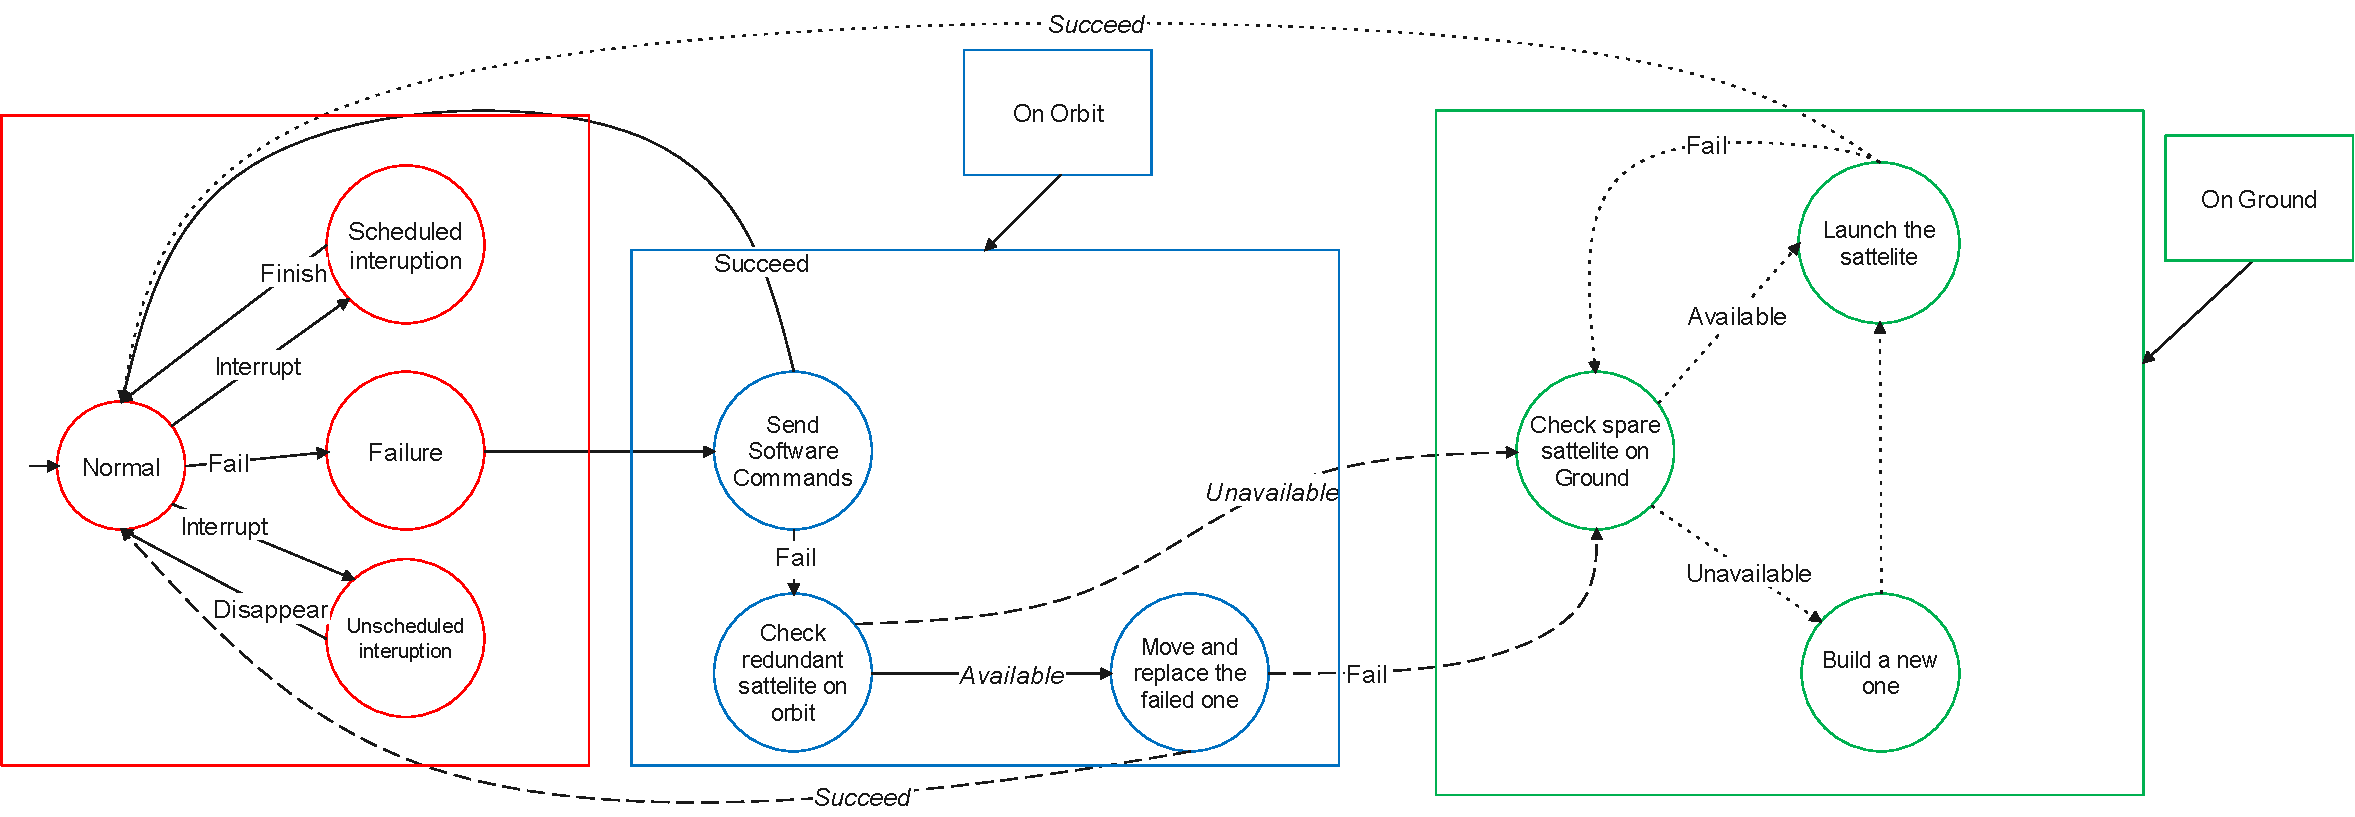
\includegraphics[width=500pt, height =180pt]{Dessin1.pdf}
    \caption{Satellite Maintenance Process Model \cite{Hoque2015,Yu2015}}
    \label{fig:usecase}
\end{figure*} 

\subsection{The system model}
This paper leverages a previously established satellite model described in \cite{Hoque2015,Yu2015,Zhaoguang2013}. The model considers the system's vulnerability to both scheduled and unscheduled interruptions throughout its lifecycle. Scheduled interruptions occur due to maintenance or software updates, leading to temporary signal unavailability for a fixed duration of \emath{t_{\alpha}=}4,320 hours. Unscheduled interruptions, such as those caused by solar radiation, can induce a Single Event Upset (SEU) in the satellite's signal. Unlike scheduled events, SEUs are unpredictable but also self-correcting, resolving automatically. Permanent failures, however, necessitate maneuvers in orbit or on the ground.


Upon satellite failure, ground and orbit control evaluate the best course of action. In some cases, the issue might be resolved remotely by sending software commands to the satellite. If the problem persists, deploying a redundant satellite from orbit as a replacement may be necessary. However, if no backup satellite is available, a new one will need to be manufactured and launched, introducing the risk of a launch failure.

The probability of a satellite failure is \emath{1-r}, where \emath{r} is its reliability calculated from the failure rate and Mean Time Between Failures (MTBF). Both the unscheduled and scheduled interruption times are \emath{t_{\alpha} = 4320 h}. If a failure occurs, there is an \emath{p_{\beta}=80\%} chance of resolving it on orbit by replacing the faulty satellite with a redundant one. If on-orbit repair is impossible, a new satellite needs to be built. The ground control team manages this process. \cmt{The times taken to decide to build a new satellite and for one to be manufactured are} \emath{t_{\gamma}=24}  hours and \emath{t_{\delta}=24}, respectively. Following a successful launch with \emath{p_{n} =90\%}, it takes another  \emath{t_{k}=24} hours for the new satellite to reach its operational position.


\subsection{On orbit and ground support capabilities}
\label{humanlabel}


The modeled system involves multiple state transitions driven by the \emph{environment}, \emph{on-orbit staff}, and \emph{ground staff}. Each group performs specific tasks:
\begin{itemize}
	\item \emph{Environment}: Triggers scheduled, unscheduled, and failure events (represented by the environment player, denoted as \emath{\mathcal{P}_{env}}) shown in red in \fig{fig:usecase}. Their actions are labeled as \emath{\alpha}.
	\item  \emph{On-Orbit Staff}: These personnel (represented by  \emath{\mathcal{P}_{o})} handle tasks like sending commands, updating software, and maneuvering the satellite into the position shown in blue in \fig{fig:usecase}. Their actions are labeled as \emath{\beta}.
	\item \emph{On-Ground Staff}:  The ground control team (represented by\emath{\mathcal{P}_{g}}) is responsible for monitoring satellite health, building new satellites when necessary, and performing launches (shown in green in \fig{fig:usecase}). Their actions are labeled as \emath{\omega}.
\end{itemize}


To model composability, we introduce a dedicated PRISM module that acts as a non-player. This module encapsulates the environment, on-orbit actions, on-ground actions, and the PRISM commands needed to synchronize their interactions. We define a CSG model, G, as a game modeling the parallel composition of the environment player \emath{\mathcal{P}_{env}}, on-orbit staff player \emath{\mathcal{P}_{o}}, and ground staff player \emath{\mathcal{P}_{g}}. This composition is coordinated by the non-player model \emath{\mathcal{P}_{\mathcal{R}}.}


\begin{mydef} \label{def:csg} \normalfont A concurrent stochastic game (CSG) for reasoning on Sattelite system maintenance is a tuple \emath{G =\gl{N, S, \bar{S}, A, \delta, AP, L}}:

\begin{itemize}
	\item \emath{N =\{\mathcal{P}_{env},\mathcal{P}_{o}, \mathcal{P}_{g}\}} is a finite set of players,

 	\item \emath{S=S_{env} \times S_{o} \times S_{g}} is a set of states, where \emath{S_{env}}, \emath{S_{o}}, and \emath{S_{g}} are states controlled by the system model, the environment model \emath{\mathcal{P}_{env}}, the on-orbit player model \emath{\mathcal{P}_{o}}, and on-ground model \emath{\mathcal{P}_{g}}, respectively \emath{\cmt{(S_{env} \cap  S_{o} \cap S_{g} =\emptyset)},}
    and \emath{\bar{S} \subseteq S } is a set of initial states,


	 \item \emath{A= A_{env} \times A_{o} \times A_{g} } where \emath{A_{env}},  \emath{A_{o},} and \emath{A_{g}} are the actions available to the environment model, on-orbit model, and the on-ground model, respectively,
    \item \emath{\delta : S \times A \longrightarrow Dist(S)} is a probabilistic transition function. Each player \cmt{\emath{\mathcal{P}_{env},\mathcal{P}_{o}, \mathcal{P}_{g}}} selects an action \emath{\alpha,\beta,\omega}, the state of the game is updated according to the distribution \emath{\delta(s, (\alpha,\beta,\omega)) \in Dist(S),} 

    \item \emath{AP} is a subset of all predicates that can be built over state variables. AP includes:
    \begin{itemize}
	\item \emath{goal}, achieved when a successful operation is reached.
     \end{itemize}
    \item \emath{L: S \longrightarrow 2^{AP}} is a labeling function that assigns each state  \emath{s \in S}  to a set of atomic propositions (\emath{AP}).
\end{itemize}
\end{mydef}


Following the definition of the CSG players, The non-player commands of \emath{\mathcal{P}_{\mathcal{R}}} that record the strategy of the CSGs model are expressed through the following transition: \emath{s_m\gparrow{\alpha,\beta,\omega}s'_m}, where \emath{\alpha} represents the label of the environment commands, \emath{\beta} denotes the on-orbit command, and \emath{\omega} denotes the on-ground commands. The non-player is modeled by the operation semantics rules \ref{s1} and \ref{s2}. The \ref{s1} is achieved by composing the modules \emath{\mathcal{P}_{env}}, \ \emath{\mathcal{P}_{o}}, and \emath{\mathcal{P}_{g}.} The \emph{standby} action refers to the idle position of the player in the CSG model. In this composition, the probability of achieving on-orbit or on-grounds tasks is determined by \cmt{\emath{\prod_{i=1}^{|N|} \lambda_{i}} such that \emath{\lambda_{i} \in \mathbb{R}}}.


\begin{figure*}[th]
\begin{boxD}
%\framedtext{
	      \begin{equation}\label{s1} \frac{ \sset{\mathcal{P}_{env}}= s_{i}\gparrow{\alpha}_{\lambda_{1}}s'_{i}  \bigwedge_{j=0}^{|A_{o}|}  \sset{\mathcal{P}_{o}}= s_{j} \gparrow{\beta_{j}}_{\lambda_{2}}s'_{j}  \wedge
       \sset{\mathcal{P}_{g}}= s_{k}\gparrow{\omega}_{\lambda_{3}} s'_{k} 
       \wedge
         \sset{\mathcal{P}_{\mathcal{R}}}= s_{m}\gparrow{\alpha,\beta,\omega}s'_{m}
       } {  \langle s_{i},\ldots,s_{j},\ldots s_{k}, \ldots s_{m},\theta\rangle  \xrightarrow{\alpha,\beta,\omega}_{\lambda_{1} \cdot \lambda_{2} \cdot \lambda_{3}}\langle s'_{i},\ldots,s'_{j},\ldots,s'_{k},\ldots,s'_{m},\theta'\rangle } \tag{\emph{On-Orbit}} \end{equation} where \emath{\alpha = Fail \wedge \omega= standby}
 
	     \begin{equation}\label{s2} \frac{ \sset{\mathcal{P}_{env}}= s_{i}\gparrow{\alpha}_{\lambda_{1}}s'_{i} \wedge \sset{\mathcal{P}_{o}}= s_{j} \gparrow{\beta}_{\lambda_{2}}s'_{j} \bigwedge_{k=0}^{|A_{g}|} 
       \sset{\mathcal{P}_{g}}= s_{k}\gparrow{\omega_{k}}_{\lambda_{3}} s'_{k} 
       \wedge
         \sset{\mathcal{P}_{\mathcal{R}}}= s_{m}\gparrow{\alpha,\beta,\omega}s'_{m} 
       } {  \langle s_{i},\ldots,s_{j},\ldots s_{k}, \ldots s_{m},\theta\rangle  \xrightarrow{\alpha,\beta,\omega}_{\lambda_{1} \cdot \lambda_{2} \cdot \lambda_{3}}\langle s'_{i},\ldots,s'_{j},\ldots,s'_{k},\ldots,s'_{m},\theta'\rangle}  \tag{\emph{On-Ground}} \end{equation} where \emath{\alpha = Fail \wedge \beta= standby}
\end{boxD}
\label{op:sec}
 \caption{Operational Semantics Rules of the CSG Game Model.}
\end{figure*}


\subsection{Measure the efficacy of collaborative maneuvers}
Measuring the efficacy of collaborative maneuvers consists of synthesizing a strategy for players \emath{\mathcal{P}_{env}}, \emath{\mathcal{P}_{o}}, and \emath{\mathcal{P}_{g}} that has the objective of reaching a state-satisfying goal and maximizes the value of the reward. The specification for the synthesis of such strategy is given as rPATL property following the pattern \emath{\mathtt{  \langle\langle\textcolor{red}{\mathcal{P}_{env}}, \textcolor{red}{\mathcal{P}_{o}}, \textcolor{red}{\mathcal{P}_{g}}\rangle\rangle} \mathtt{ P=? [ F} \ goal\mathtt{]}} where \emath{goal=(}\quot{\emath{\textcolor{red}{win}}}\emath{\& \ \textcolor{red}{rounds}<=\textcolor{red}{k})} to quantitatively evaluate the efficacy of collaborative maneuvers to the round \emath{k}. However, to calculate the reward or cost related to collaborative maneuvers it will take the following pattern: \emath{\mathtt{  \langle\langle\textcolor{red}{\mathcal{P}_{env}}, \textcolor{red}{\mathcal{P}_{o}}, \textcolor{red}{\mathcal{P}_{g}}\rangle\rangle}} \emath{\mathtt{R\{}}\quot{\textcolor{red}{win}}\emath{{\}=?[F } \ goal\mathtt{]}} where \emath{goal} =(\emath{\textcolor{red}{rounds}<=\textcolor{red}{k}}). In this case, the reward reflects the number of times the collaborative maneuvers wins the game within a specific round  \emath{k.}